\chapter{Analysis of iris obfuscation: Generalising eye information processes for privacy studies in eye tracking}

\section*{Overview for the thesis}

\emph{
The experimental part of this thesis is largely contained in the following article, which proposes and evaluates a large number of possible iris obfuscation methods. Iris obfuscation is concerned only with the selective degradation of iris patterns in eye-tracking. The term is first used in (REF) where a simple low-pass filter model is presented using either optics or convolution but is expanded in the article to cover more general cases using the EIP model terminology. }

\emph{The article presents a short overview of some of the same points made in this thesis. Afterwards, the obfuscation methods are introduced and tested in two different experiments to first determine appropriate method parameters and subsequently evaluate the actual performance. It presents both the EIP model and large-scale evaluation as contributions bringing the field towards a better base for understanding iris obfuscation methods, difficulties, and limitations. Additionally, some of the presented methods outperform existing ones by a large margin. These have been defined as a result of the analysis presented here and in the article and are therefore also used as arguments for the models usefulness for this application.}

\emph{The technical details and further analysis and discussion of the results are presented in the next chapter to better tie the article's narrative into this thesis.}


\begin{figure}[b]
    \centering
    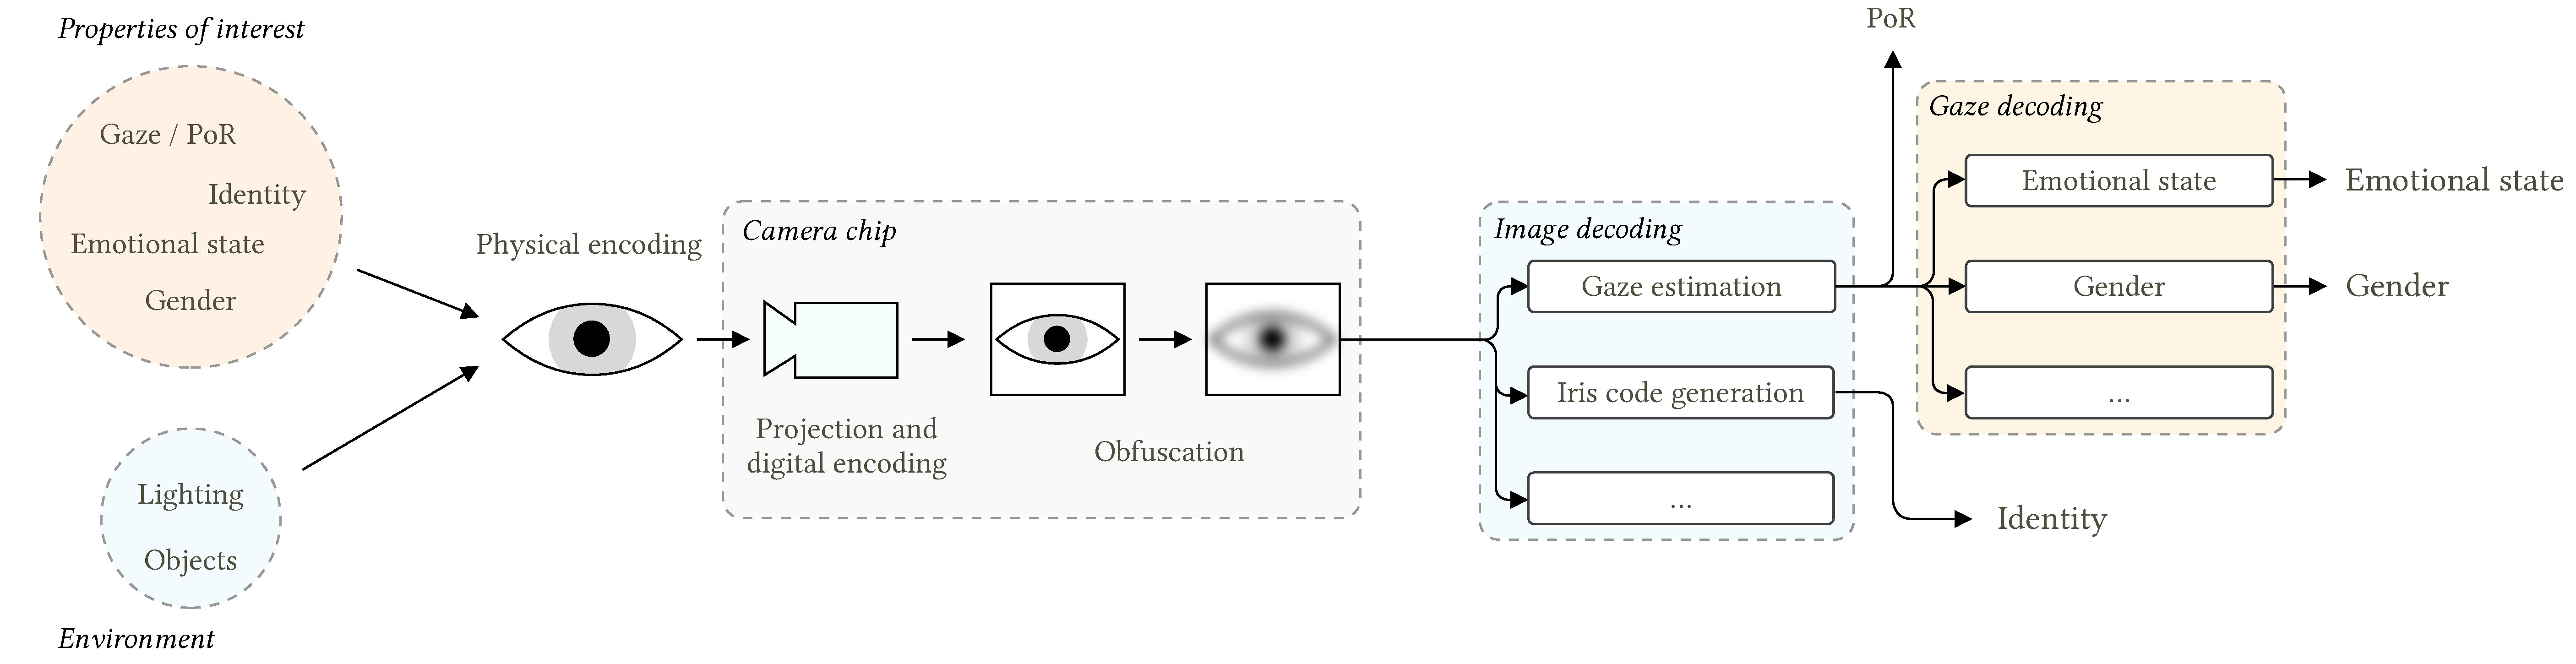
\includegraphics[width=1\textwidth]{figures/Model.pdf}
    \caption{Eye information model.}
    \label{fig:overview}
\end{figure}


\section{Introduction}
It is well known that eye tracking data, including images and gaze signals, can be used in identification of mental and physical traits including a persons identity. This is cause for concern due to the increasing prevalence of products using eye tracking technologies and availability of eye tracking datasets.

\emph{Iris recognition} in particular is of concern due to the maturity, availability, and high accuracy of existing methods. The human iris is ideal for personal identification because it exhibits three very important characteristics. (1) The iris pattern which is created by complex interactions between light and the fibrous stroma is highly variable across large populations. (2) Although genes do affect the development of certain iris pattern characteristics, they are generally considered to develop randomly (or as a response to the environment) during development - therefore identical twins and even individual's left and right eyes differ significantly. (3) Iris patterns are stable throughout life. Iris recognition is one of the strongest known biometrics (ref) with state of the art studies reporting \emph{false acceptance rates} (type II error) of at most $2\times 10^{-10}$\cite{DAUGMAN_NEW}. Because head-mounted eye trackers typically capture images where the iris has a high resolution (caused by the eyes proximity to the camera), the images can be reliably used for iris recognition \cite{BRENDAN_BLUR}. 

The possibility of personal identification from eye tracking products has both potential legal and ethical implications. For example, the GDPR (general data protection regulation) regulation defines personal data as including ``any information relating to an identified or identifiable natural person'' \cite{eu-gdpr}. Here, \emph{identifiable} person is defined as ``any person who can be distinguished from others'' \cite{eu-gdpr}. In other words, iris patterns are covered by the GDPR since they can be used to discover the identity of a person. This has the potential to increase the difficulty and feasibility of using eye tracking in both research and consumer products due to the added complexity of handling personal data. From an ethical standpoint this is also a problem of users or participants knowing what information they are actually sharing about themselves. In this age of large-scale data collection, being able to very accurately link other behaviours to identities has to be taken seriously.

The iris pattern data itself is not necessarily directly used by the eye tracking system itself. Therefore, a possible solution to this set of problems is to alter the eye images in a manner that decreases the accuracy of iris recognition while causing minimal impact to the estimation of gaze. We use the term \emph{iris obfuscation} for this task. For applications in consumer and commercial products, implementations of obfuscation should ensure that the original, unmodified image can never be accessed. This is only possible if the obfuscation method is built into the source camera. Due to both physical limitations and cost considerations, practical obfuscation methods should therefore be as simple as possible. 

Currently, no comprehensive overview and comparison of existing and new methods exist. A number of studies using optical defocus (and Gaussian filters) \cite{BRENDAN_BLUR, BRENDAN_ARTICLE} and salt-and-pepper noise \cite{BRENDAN_SNOW} have shown promising results but lack large-scale testing of iris recognition performance and method comparisons. A comparison study does exist \cite{IRIS_OBF} but it is focused on methods that require detection of the iris itself which, for the purposes of this paper, is considered to be outside the reasonable expectations for cheap embedded implementations in eye tracking systems. Additionally, the study does not consider gaze estimation accuracy. 

This paper presents a comprehensive study of a number of existing and new methods for iris obfuscation that are all based on image filters and noise functions. Of the proposed methods, the \emph{bilateral filter} achieves the highest rate of obfuscation with a measured \emph{false rejection rate} of $??\%$ at a mean relative gaze error of $1$ compared to the baseline. This is xx lower than xx and so on. Additionally, we propose the use of a communication model as the basis for understanding and evaluating the behaviour of iris obfuscation methods without relying on specific implementations for iris recognition and gaze estimation. Finally, we discuss the actual level of anonymity the shown methods provide depending on the use case. This also includes an examination of the differential privacy based approach in\cite{BRENDAN_SNOW}.

\subsubsection{Overview}
This work is comprised of two experiments. Both use individual datasets for gaze estimation, pupil detection, and iris recognition. The first experiment concerns discovery of optimal parameters for the presented obfuscation methods. and how small parameter changes impact gaze accuracy and iris recognition. It uses smaller samples from each dataset to estimate a number of metrics for each parameter configuration. The results provide insight into how the methods affect the images and how these changes are connected to each metric. Additionally, the results are used to select a small number of interesting configurations for further testing. The second experiment tests these configurations on the entire datasets. The results of this experiment includes a complete cross-comparison of $2,226$ samples from the CASIA IV (REF) dataset. 

\section{Related work}
This work aims to improve the status quo and provide a more comprehensive overview of iris obfuscation methods used in research so far. Related work therefore includes other obfuscation methods as well as methods in image and signal processing, information theory, and differential privacy.

As mentioned, obfuscation of iris patterns has previously been attempted (REFS). (REF) presented the initial claim that a low-pass filter would be able to selectively obfuscate the iris pattern while still being able to detect eye features (pupil and corneal reflection) in the image. This is based on the notion that an image $I$ can be decomposed into an iris component $I_R$ and a feature component $I_C$ such that $I=I_R+I_C$. This has inspired the communication model and use of mutual information in this paper although we make several extensions to allow its use in evaluation of the proposed iris obfuscation methods. Additionally, we challenge the study's claim that $I_C$ is dominated by low frequencies in the frequency domain by demonstrating how the bilateral and non-local-means filter which are selective low-pass filters, both outperform Gaussian blurring in our tests. A later study (REF) uses a salt-and-pepper like filter named \emph{snow} to perform iris obfuscation which is also included in the tests presented here. The study also presents a model for how the method could be implemented in hardware and thus shares our sentiment of the importance of isolation.

Image 




\section{A model for eye information}
This section introduces a probabilistic model for understanding \emph{eye processing systems}. An eye processing system is any software and/or hardware system which uses eye image capture to extract information about its subjects. It therefore covers both gaze estimation and iris recognition. The purpose of the proposed model is to allow reinterpretation of gaze estimation, iris recognition, and potentially other eye information processes under a common frame of reference. This makes it easier to understand how potentially conflicting goals such as iris obfuscation and gaze estimation interact and what trade-offs between them are likely to occur. Our hope is that the model will be used as a point of reference and comparison for future studies in this field.

%This allows analysis of how different goals affect each other. In the context of this paper, it specifically provides a framework for understanding how 

%This section presents a model and a methodology for understanding eye information processes. 
%This section presents an overview of the model used throughout the paper to examine the processes of iris recognition and gaze estimation from a common frame of reference. This allows critical analysis 





%This section presents a model for understanding how information flows through such systems and how image manipulations affect the information measurement processes. This allows us to evaluate and compare the obfuscation methods from a purely theoretical perspective which ... \todo{Overvej integration.. hvad giver det her? }

Any eye processing system has the goal of accurately measuring some properties of the real world through capture of eye images. These properties are encoded through physical processes as signals which are transformed and processed with the goal of isolating the property of interest from everything else. The systems therefore essentially have the function of signal denoising, albeit rather aggressively because anything but the target property is considered noise. Similarly, eye processing systems comprise a communication channel pipeline, with each physical encoding, image capturing, or transformation process forming a component in the pipeline. We propose a probabilistic graphical model which allows interpretations from both perspectives. 

%Similarly, information theory lets us define image processing as a communication system and analyse how uncertainty propagates and is added from noise. This lets us evaluate the effect of obfuscation methods directly on the image data. Although this is not in itself enough to demonstrate the effectiveness of the proposed methods, it creates a reference frame that does not depend on specific implementations of any algorithms. We propose a model which allows useful interpretations from both points of view and which has a simple graphical representation (shown in \autoref{fig:model}).

\begin{figure}
    \centering
    \begin{tikzpicture}[node distance=1.3cm]
        \node (q1) [] {$Q_1$};
        \node (qd) [right of=q1] {$\dots$};
        \node (qn) [right of=qd] {$Q_n$};
        \node (t1) [align=right, left of=q1] {(1)};
        
        %\node (e1) [rect, below of=q1] {$f_e^{(1)}$};
        %\node (ed) [right of=e1] {$\dots$};
        %\node (en) [rect, right of=ed] {$f_e^{(n)}$};
        %\node (t2) [align=right, left of=e1] {(2)};
        
        
        %\draw [arrow] (q1) -- (e1);
        %\draw [arrow] (qn) -- (en);
        
        \node (c) [rect, below of=qd] {$f_e$};
        \node (t3) [align=right, below of=t1] {(3)};
        \draw [arrow] (q1) -- (c);
        \draw [arrow] (qn) -- (c);
        
        \node (f1) [rect, below of=c] {$f_p$};
        \node (fd) [below of=f1] {$\dots$};
        \node (fn) [rect, below of=fd] {$f_n$};
        \draw [arrow] (c) -- node[anchor=east] {I} (f1);
        \draw [arrow] (f1) -- (fd);
        \draw [arrow] (fd) -- (fn);
        
        \node (t4) [align=right, below of=t3] {(4)};
        
        \node (dd) [below of=fn] {$\dots$};
        \node (d1) [rect, left of=dd] {$f_d^{(1)}$};
        \node (dn) [rect, right of=dd] {$f_d^{(n)}$};
        \node (t5) [align=right, left of= d1] {(5)};
        
        \draw [arrow] (fn) -- node[anchor=south east] {$I^*$} (d1);
        \draw [arrow] (fn) -- node[anchor=south west] {$I^*$} (dn);
        
        \node (r1) [below of=d1] {$R_1$};
        \node (rd) [right of=r1] {$\dots$};
        \node (rn) [right of=rd] {$R_n$};
        
        \draw [arrow] (d1) -- (r1);
        \draw [arrow] (dn) -- (rn);
    \end{tikzpicture}
    
    \caption{Eye information processing model: (1) Input properties. (2) Functions that encode the physical manifestation and uncertainties of the source properties. (3) Image capturing process. (4) Image processing steps which may typically be described as a single function. (5) Decoding functions that aim to extract original properties, e.g. an iris pattern or gaze direction.}
    \label{fig:model}
\end{figure}


%We define a model that allows easy analysis from both a signal-processing centric and probability centric view. 

Let an eye information processing system be defined by $\Lambda = \{Q, R, f_e, \mathcal{D}, \mathcal{P}\}$, where $Q=\{Q_1, \dots, Q_n\}$ is a set of source properties, $R=\{R_1,\dots,R_n\}$ is a set of output properties, $f_e$ is an encoding function, $\mathcal{D}=\{f_d^{(1)}, \dots, f_d^{(n)}\}$ is a set of decoding functions, and $\mathcal{P}=\{f_p^{(1)}, \dots, f_p^{(n)}\}$ is a set of processing functions. A graphical representation is shown in \autoref{fig:model}. The encoding functions in $f_e$ represent how properties are manifested as physical quantities and captured by a camera. This simplification retains the modelling of uncertainty in both processes. The results are given as $R_i = (f_d^{(i)}\circ f_p)(\hat{Q})$. To encode noise and information loss, all properties and functions are viewed as discrete signals composed of random samples of some distribution. The terms signal and property are therefore used interchangeably throughout this text.

%To show this, note that a graph is defined by $G=\{V, E\}$ which in this model is given by $V = Q\cup R\cup \hat{Q}$ and $E = \mathcal{E}\cup \mathcal{D}\cup \mathcal{P}$. %It will not, however, be used to infer conditional probabilities but, as stated earlier, to understand how uncertainty propagates through the system.

%The purpose of the model is to make inquiries about decoding uncertainties and signal correlations intuitive and generalisable. For example, the noise resulting from an iris encoding is given by $P_{R_{iris}|Q_{iris}}$


\paragraph{Model analysis}
This section presents some fundamental definitions from information theory and signal processing that are necessary to describe and analyse iris recognition, gaze estimation, and iris obfuscation from the perspective of the graphical model.

Information theory enables precise definitions for the uncertainties retained and introduced at all parts of the presented model. The base measure is entropy, denoted $H$ which defines the optimal average encoding length of symbols $x_i$ drawn from a discrete distribution $X$ defined by
\begin{align}
    H(X) = -\sum_{x\in \mathcal{X}} p(x)\log_2p(x),
\end{align}
with results in the units of bits. Different bases may be used for alternate units. A uniformly distributed random variable has the maximum entropy for its number of states, precisely $\log{N}$. In terms of iris recognition, the entropy of code symbols (bits are typically used) can be used to calculate the expected amount of information present in the entire signal. For example, Daugman calculated the expected iris code entropy by fitting a binomial distribution to the iris code distance comparisons, which revealed an approximate 250 bits of information between codes (REF). This entropy only accounts for the information content in the final codes and thus does not account for noise added during the encoding and processing steps. 

Mutual information is a measure that defines exactly how much entropy is preserved over a communications channel and is thus useful for determining how much information is actually captured by a specific process. Its definition is 
\begin{align}
    I(Y;X) = \sum_{x\in \mathcal{X}, y\in \mathcal{Y}} P_{X,Y}(x, y)\log_2 \frac{P_{X,Y}(x, y)}{P_{X}(x)P_{Y}(y)} = H(Y) + H(Y|X),
\end{align}
where $H(Y|X)$ is the conditional entropy which is a measure of the error added by the communication channel.

\begin{align}\label{eq:entropy-law}
    H(X) = I(Y;X)+H(Y|X)
\end{align}

For iris obfuscation, the goal is to minimise $I(R_{iris}, Q_{iris})$ and maximise $I(R_{gaze}, Q_{gaze})$. Measuring these directly is again not possible as the $Q$ signals are not the measured signals. The only known information source is the image $I$ where the two signals have been combined into a single signal. However, because $H(Q_{gaze})$ should be very low, i.e. it represents an encoding of just two decimal values, the mutual information between the original and obfuscated images $I(I, I^*)$ can be used as a proxy to measure the level of obfuscation. Additionally, for any set of signals $X, Y, Z$ where $Z = f_z(Y)$ and $Y= f_z(X)$, then $I(Z; Y) \leq I(Z;X)$ (REF to proof). Thus, it is an upper bound for the mutual information which makes the results much more useful.

Finally, the notion of channel capacity is used to define the maximum mutual information of a communications channel for any input distribution. It is defined as
\begin{align}
    C = \sup_{p(x)} I(X, Y).
\end{align}
The channel capacity of specific obfuscation methods define strong upper limits on the amount of information that is able to pass. If an obfuscation method has capacity below the minimum requirement for differentiation of a population given the optimal distribution (uniform), it is impossible to accurately differentiate between all individuals. In practice, however, the image signal which is measured contains orders of magnitude more information, making such guarantees unlikely, at least for the methods presented in this paper. Instead, we use the measure to evaluate the relative obfuscation of information.



\subsubsection{Measuring information in images}
The term signal is rather abstract but is typically defined as a function that encodes or contains information of interest. Signals can be defined over temporal inputs, spatial inputs, or both. In the case of eye information processes, signals such as the captured eye images may be analysed individually as purely spatially divided signals or jointly as a time series of frames. The iris pattern in either its abstract or encoded form, is only resolved spatially while the gaze signal is usually analysed as a time-series. 




When viewed as bandlimited discrete signals of two dimensions, images can be analysed structurally through the 

To measure entropy and mutual information in images, it is necessary to formulate a method for defining the image in terms of a probability distribution. Specifically, it is necessary to define a model for the image distribution and estimate it using the image itself as data.

The fundamental model is that each image can be represented by an unknown distribution $P_{img}$ of an unknown number of random variables $X^1, \dots, X^n$. A simple model is the intensity histogram which estimates a discrete distribution of intensity values assuming that each pixel is independent of each other. It can be defined as
\begin{align}
    P(I=i) = \sum_{x\in\mathcal{X}y\in\mathcal{Y}} \delta_{i, I_{x,y}},
\end{align}
where $\delta_{a, b}$ is the Dirac delta function. The downside to this approach is that no correlations between pixels are considered even though they clearly exist. For use in obfuscation measurement, this is problematic since the iris recognition methods use texture and not direct pixel intensities for detection. 

In the most general terms, the distinct features of an iris pattern represents differences in the amplitude and phase of different frequencies. Many iris algorithms of the Daugman type use spatial phase responses to calculate a robust iris code. These traditional methods generally use some form of wavelet transform to separate spatial frequency-responses (REFS). The convolutional neural-network based methods likely learn similar approaches as they have been shown to learn typical bandpass-filters like the wavelets used by Daugman (REF). 

The image derivative, defined by its two partials, has excellent properties for measuring image texture complexity. The image derivative retains all information necessary to reconstruct the original image and is therefore still a valid upper bound on information measures (REF). By defining $P_{img}$ as a joint distribution of the partial derivatives of the image
\begin{align}
    P(dx=i, dy=j) = \sum_{x\in\mathcal{X}y\in\mathcal{Y}} \delta_{i, {I_{\Delta x}}_{x,y}} \delta_{j, {I_{\Delta y}}_{x,y}},
\end{align}

Additionally, we also define joint distributions on convolutions with complex Gabor wavelets. A Gabor wavelet works as a bandpass filter, i.e. it responds only to certain frequency ranges. Defining a joint distribution over the Gabor response of a particular filter makes it possible to measure the entropy in certain frequency ranges which further... By definition however, a bandpass filter does not retain all the information in the original signal and can therefore not be used for definition of upper bounds.





\section{Common reference frame}
The systems of interest in this paper are iris recognition, gaze estimation, and obviously iris obfuscation. Understanding how they are connected theoretically is critical in choosing suitable obfuscation methods and analysing the impact of the results...


\paragraph{Iris recognition}
Using the definition of an eye information system, iris recognition can be defined as the task of determining the probability of two iris codes $R^a$ and $R^b$ originating from the same source signals $Q^a = Q^b$ or different source signals $Q^a\neq Q^b$. Iris code is here used as a general term to cover any signal used for iris comparison. The probabilities are defined as $P(Q^a\neq Q^b|R^a, R^b)$, $P(Q^a\neq Q^b|R^a, R^b)$ and are determined by the comparison algorithm used. These are typically inferred by creating a distance metric $S = h(R^a, R^b)$ which is used for estimating the proxy distributions $P(S|Q^a\neq Q^b)$ or $P(S|Q^a\neq Q^b)$. In the most traditional case, iris recognition acceptance is performed by failing a statistical test of significance, i.e. determining that $P(S|Q^a\neq Q^b)$ is extremely unlikely. This was first proposed by Daugman (REF) and can be reformulated as
\begin{align}
\begin{aligned}
    h_0: & \quad s = h(R^a, R^b) &&\sim  P_{S|\hat{Q}^a\neq \hat{Q}^b}\\
    h_1: & \quad s && \sim  P_{S|\hat{Q}^a = \hat{Q}^b}.
\end{aligned}
\end{align}

In terms of the proposed eye information model, these distributions depend only on the internal system noise. 

We assume the original iris distribution to be uniform, i.e $P(Q)=1/N$ where $N$ is the total population. Given zero noise, $H(R|Q)=0$ and $H(R)=H(Q)$, $P(R)$ must be uniform on its support. As a result, $S$ which is defined to be $0$ when $R^a = R^b$, must have $P(S=0|Q^a = Q^b)=1$ and $P(S>0|Q^a \neq Q^b)=1$ since the original signals completely determine $S$. 

Because $S$ is bounded (here assumed to be normalised), an increase in noise $H(R|Q)$ increases the variance of $S$. Formally, as the noise approaches the maximum entropy of $R$, given by $M$, the distribution of $P(S)$ is
\begin{align}
\lim_{H(R|Q)\rightarrow M} P(S) = U(0, 1),
\end{align}
where $U(0, 1)$ denotes a discrete distribution of $M$ possible outcomes normalised to values in the $]0, 1[$ range. In the opposite direction, information may be lost due to low resolution image capture or bad decoding methods. This is represented by $I(R;Q)$. The relation in \autoref{eq:entropy-law} shows that mutual information limits the amount of information transmitted through the system. The limit is
\begin{align}
\lim_{I(R;Q)\rightarrow 0} P(S) = 0.
\end{align}

In other words, iris recognition systems are limited by their ability to transmit the iris pattern without introducing noise or capturing too little detail.

\paragraph{Gaze estimation}
Gaze is defined as either the direction or point of visual attention of a given subject. This property is by definition at least partially subjective, as the point of attention does not always coincide with the fovea, but instead is at least partially controllable by the subject (REF). The physical encoding of gaze is then, at least when only observing the eye's immediate position and orientation, inherently probabilistic. This is captured by the model as the distribution $P(\hat{Q}|Q_{gaze})$, if the encoding function is split between physical encoding and image capture such that $I=f_{capture}(\hat{Q})$ and $\hat{Q}=f_{physical}(Q_{gaze}, \dots)$. 

Each additional step in a given gaze estimation system introduces some amount of additional noise given by its imperfections. Robust gaze estimation can therefore be defined as transformations and decoders that have low noise-rates for large variations in signal distributions. Consequently, a non-robust system is characterised by having low noise-rates only for a narrow subset of input signals. 

%$P(I^{*1}|I^*),\dots, P(I^{*n}|I^{*(n-1)})$


\begin{align}
    \min ||Q_{gaze} - f^{gaze}_d \circ f_p^{(n)} \circ \dots \circ f_p^{(1) \circ f_e}(Q)||_2
\end{align}


\paragraph{Obfuscation}
This article's definition of iris recognition provides two paths that enable obfuscation. Increasing noise makes accurate recognition harder, while decreasing mutual information makes differentiating between irises more difficult. Artificial noise is easily added to signals using pseudo-random number generation. Mutual information decrease can be performed by either literally removing signal pieces or by using low-pass filters to remove detail. Because of the relationship between noise and mutual information (\autoref{eq:entropy-law}), adding noise also negatively affects mutual information... Thus, the expected level of obfuscation can be measured by...



To limit or prevent iris recognition, the internal noise measured as $H(R^{iris}|Q^{iris})$ should be increased towards the entropy limit. Obviously this goal is countered by the needs of gaze estimation, which require a low $H(R^{gaze}|Q^{gaze})$. Thus, obfuscation should selectively increase 

We define obfuscation as a minimisation of mutual information between the original and modified images subject to

\begin{align}
\begin{aligned}
    &\min & & \mathcal{I}(I, I^*)\\
    &\text{subject to } & &  \frac{J_{gaze}(I)}{J_{gaze}(I^*)} \leq t,\\
    \text{where:}&\\
    &&J_{gaze}(x) =& ||Q_{gaze}- f_d^{(gaze)}(x)||\\
    &&I =& \left( f_p^{(n-1)} \circ \dots \circ f_p^{(1)} \circ f_e\right) (Q)\\
    &&I^* =& f_p^{obf}(I)
\end{aligned}
\end{align}

Here, $t$ is an arbitrary threshold.

Iris recognition and gaze estimation have similar ideal physical setups. High-resolution images taken in controlled lighting conditions (typically using infrared lighting) are ideal in both cases. 

%In terms of this model, iris recognition is the process of determining whether two encoded iris signals $R^a$ and $R^b$ originate from the same source iris signal $\hat{Q}^a=\hat{Q}^b$ or from different signals $\hat{Q}^a\neq \hat{Q}^b$. Since $\hat{Q}$ cannot be known directly ($R$ is our best approximation) the goal must instead be expressed in terms of the detected iris codes. In order to provide some form of comparison, a distance function $S = h(R^a, R^b)$ is added. $P_{S|\hat{Q}^a\neq \hat{Q}^b}$ can be estimated directly from data and used in a test of statistical significance to determine whether a specific distance $s$ is unlikely to have been caused by different iris patterns. The hypothesis is




%When interpreting source and encoded iris signals as some fixed $n$-sample of probability distributions $P(Q^a)$ and $P( C^a )$ respectively, their information content is determined by the Shannon entropy measure defined as
%$$
%H(X) = -\sum_n p(x)\log_2p(x)
%$$
%This measure determines, in bits, how much information is actually present in the signal. This is important when we want to use the signals for unique identification. Assuming we can use the source iris signal $Q$, which here is defined as an abstract notion of a signal perfectly capturing the physical information in a given human iris, the average signal entropy needs to be at least 
%$$
%\frac{1}{N}\sum_{n\in \hat{Q}}H(Q^a) \geq \log_2 N
%$$
%where $N$ is the number of unique identities. Of course, it is impossible to capture $Q$ and even then the iris is still subject to small changes which adds noise. This noise may be modelled by assuming a true unchanging identity $P$ which through various physical processes result in a physical iris manifestation $Q$ as shown below:

%The source properties are encoded by $f_e$ as signals $\hat{Q}=\{Q_1, \dots, Q_n\} = f_e(q_1, \dots, q_n)$. These are captured by a camera to form the image signal $I=f_c(\hat{Q})$. An image processing function representing the obfuscation operation $I^* = f_p(I)$. The properties are then recreated by $r_i = f_d^{(i)}(I^*)$

%and $f$ is a function of $\hat{Q}$, $f(\hat{Q}) = \hat{R}$. $f$ represents the encoding, capture, and processing of the source signals. To better differentiate between the stages, we split $f$ into an encoding function $f_e$, a processing function $f_p$, and a decoding function $f_d$ such that $f=f_d\circ f_p \circ f_e$. Thus the encoding function represents both the physical manifestation of each signal as well as the camera's capture. The processing function is here used primarily to signify the obfuscation method. The decoding function then comprises everything else necessary for decoding a given signal. 


%Let an eye information processing system be defined by $\Lambda = \{\hat{Q}, \hat{R}, f\}$, where $\hat{Q}=\{Q^1, \dots, Q^n\}$ is a set of source signals, $\hat{R}=\{R^1,\dots,R^n\}$ is a set of output signals, and $f$ is a function of $\hat{Q}$, $f(\hat{Q}) = \hat{R}$. $f$ represents the encoding, capture, and processing of the source signals. To better differentiate between the stages, we split $f$ into an encoding function $f_e$, a processing function $f_p$, and a decoding function $f_d$ such that $f=f_d\circ f_p \circ f_e$. Thus the encoding function represents both the physical manifestation of each signal as well as the camera's capture. The processing function is here used primarily to signify the obfuscation method. The decoding function then comprises everything else necessary for decoding a given signal. 

%A signal represents a specific 

%The signals are random variables, instances of which are also random variables. E.g. $Q^1$ might represent an identity, $P(Q^1)$ the distribution of all identities, and $Q^1_1$ is ... 


%Images are often described as two-dimensional band-limited signals (ref). They are effectively the result of transmitting a source image signal consisting of photons over a communication channel which turns the photons into an image, i.e. a camera. In the same manner, any image manipulation is also a channel which transmits the image and possibly other signals.

%Let $\Lambda = \{\hat{Q}, \hat{O}, E, D,  f\}$ be an image communication system where $\hat{Q}$ is a set of source signals, $\hat{O}$ is a set of output signals, $E$, $D$ are encoding and decoding functions respectively, $X=E(\hat{Q})$ and $f$ is a channel which receives the encoded signal $X$ and emits $Y$.
%\begin{equation}
%    \Lambda = \{\hat{Q}, \hat{O},  \}
%\end{equation}





%To analyse the bounds on entropy necessary for accurate identification of $P$'s given $Q$'s, we need to first introduce a few notions from information theory. While entropy measures the uncertainty  in a single signal, mutual entropy $I(X, Y)$ measures the uncertainty shared between signals $X$ and $Y$. Another measure, conditional entropy $H(Y|X)$ measures the uncertainty of $Y$ after $X$ has been observed. The two measures can be defined in terms of each other $I(X, Y) = H(Y)-H(Y|X) = H(X) - H(X|Y)$. When $Y$ is produced by a communications channel from $X$, conditional entropy describes the noise added from the channel itself, while mutual information describes the entropy caused by the source signal.

%This leads to the notion of *channel capacity* which is the upper bound of mutual information through a channel for any distribution of the input signal. It is defined as
%$$
%\mathcal{C} = \sup_{p(x)} I(X, Y)
%$$
%We use a special font for $\mathcal{C}$ to distinguish it from iris code signals %$C$. For our iris recognition system we can add as a requirement that
%$$
%\frac{1}{N}\sum_{P\in\hat{P}} I(P, Q) \geq \log_2 N
%$$
%This is a tighter bound than the last one since $I(X, Y) \leq H(X)$ by the definition of mutual information.





%\subsection{Unknown}
%Look at the sample image. Features used for gaze estimation are really clear while features used for iris recognition are subtle and unpredictable. Depending on the algorithm, more than just the pupil and glints may be used for gaze estimation...



%Understanding images as bandlimited signals. We are essentially capturing an oscillating random variable which can be expressed as an infinite sum of sine waves (fourier series). This is important because it gives us more insight into what we can actually capture.

%First of all, the nyquist frequency dictates the smallest features (or frequencies) we can accurately detect - this is another way of explaining how and why image resolution matters when trying to capture a pattern (iris).

%Secondly, the features directly (or indirectly) used for gaze estimation (pupil + glints), are neither low nor high-frequency features. Instead, they look like steep, almost vertical, rises and drops, akin to square waves. As we know, these are created by adding (something) together and these features thus span the whole frequency range! This is important when choosing suitable obfuscation methods.
% \chapter{Method}
This chapter presents additional details on the experimental work performed as part of this thesis. It builds directly on the material presented in the article, which describes only the most relevant and critical details. Additional results and experiments are presented in the next chapter.

The primary contribution of this work in terms of implemented software, is the platform designed and created for the experimental work presented in the article. The platform consists of tools for optimisation, entropy calculations, iris recognition, gaze estimation as well as a platform for defining, running, and analysing iris obfuscation experiments. 


\section{Implementation details}
This section presents the scope and important details of the software systems implemented to achieve the goals...

FIGREF shows a high-level diagram of the provided software. 

T


\subsection{Optimisation engine}
In order to support different approaches to optimisation, the component has been designed such that any form of optimisation may be implemented. 

The MultiObjectiveOptimizer class expects an Objective and produces a set of results by calling its run method. The run method is implemented differently for each subclass to support different types of optimisation. The NaiveMultiObjectiveOptimizer does not use feedback for determining parameters for the next iteration and instead relies on sampling based parameter selection - this is the class used in the experiments. Additionally, a PopulationMultiObjectiveOptimizer is an implementation of the so called \textit{vector evaluated genetic algorithm}, which uses population strategies to combine and select parameters. The method is discussed in further detail in SECREF, where its possible uses for future work is considered.

Each optimiser has exactly one Objective. The abstract Objective class only has a single sub-class ObfuscationObjective for now but additional ones would be necessary for other optimisation methods or other optimisation tasks. The purpose of the Objective class is to calculate a set of Metrics given a set of parameters. In ObfuscationObjective this is done as described in the article by using different datasets for different metrics. 

Specifically, the objective object is initialised with a pool of datasets divided into three categories: Iris datasets, Gaze datasets, and pupil centre datasets. As seen on the class diagram, this terminology arises from the fact that the gaze datasets are subdivided. The objective can be initialised with any number of different metrics provided as objects. Calling the \emph{eval} function results in the metrics being calculated for a number of samples drawn from the datasets. The sample size is determined at the moment of initialisation.

Results are recorded in a special Logger object, which wraps a dictionary and provides convenient methods for accessing the data.

\subsection{Interactive tools}
\begin{figure}
	\begin{subfigure}{0.3\textwidth}\centering
		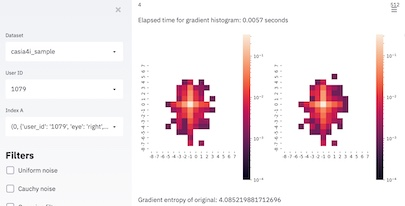
\includegraphics[width=1\linewidth]{figures/labs/EntropyLab}
		\caption{Entropylab}\label{fig:tools:entropylab}
	\end{subfigure}
	\hfill
	\begin{subfigure}{0.3\textwidth}\centering
		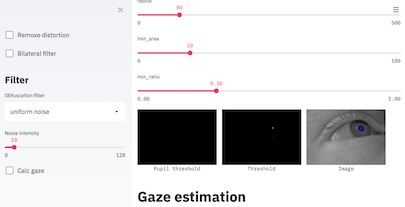
\includegraphics[width=1\linewidth]{figures/labs/GazeLab}
		\caption{GazeLab}\label{fig:tools:gazelab}
	\end{subfigure}
	\hfill
	\begin{subfigure}{0.3\textwidth}\centering
		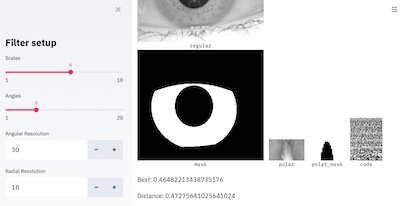
\includegraphics[width=1\linewidth]{figures/labs/ObfuscationLab}
		\caption{ObfuscationLab}\label{fig:tools:obfuscationlab}
	\end{subfigure}
	\\
	\begin{subfigure}{0.3\textwidth}\centering
		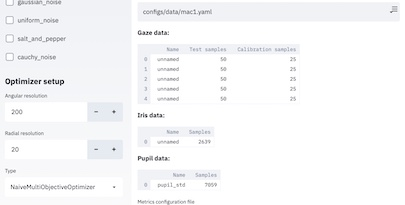
\includegraphics[width=1\linewidth]{figures/labs/OptimisationLab}
		\caption{OptimisationLab}\label{fig:tools:optimisationlab}
	\end{subfigure}
	\hfill
	\begin{subfigure}{0.3\textwidth}\centering
		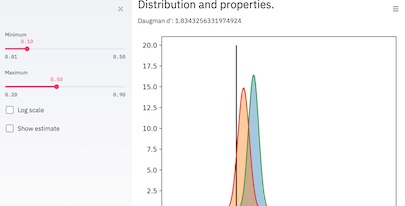
\includegraphics[width=1\linewidth]{figures/labs/ObfuscationResultAnalyser}
		\caption{ObfuscationResultAnalyser}\label{fig:tools:obfuscationresultanalyser}
	\end{subfigure}
	\hfill
	\begin{subfigure}{0.3\textwidth}\centering
		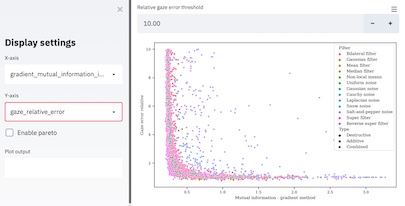
\includegraphics[width=1\linewidth]{figures/labs/OptimisationResultAnalyser}
		\caption{OptimisationResultAnalyser}\label{fig:tools:optimisationresultanalyser}
	\end{subfigure}
	
	\caption{Screenshots showing the individual interactive tools. The code is, of course, included with the thesis submission as well.}\label{fig:tools}
\end{figure}

In terms of the optimisation experiment described in the article, each obfuscation method represents one MultiObjectiveOptimizer instance. To make experimentation and repeatability easier, a number of interactive tools are created using StreamLit which is a Python library for creating data-rich, interactive, web applications.

Six different interactive tools were created - some for experimenting with 
\begin{description}
	\item [EntropyLab] Tool for experimenting with image-based entropy measurements and their distributions.
	\item [GazeLab] Tool for experimenting with gaze estimation parameters and evaluating performance.
	\item [ObfuscationLab] Explorative tool for testing the iris obfuscation algorithm and setting up configuration files for large-scale testing. 
	\item [OptimisationLab] Tool used for running small optimisation experiments and creating configurations for larger ones. 
	\item [ObfuscationResultsAnalyser] For testing the result of running the iris obfuscation experiment. Only allows simple analyses and was mostly used during development of the iris recognition algorithm to test performance.
	\item [OptimisationResultsAnalyser] Detailed interactive analysis for the parameter experiments. It has been used primarily to discover interesting facets of the results. Due to the large number of metrics used for analysis, interactive visualisations provide....
\end{description}


\section{Gaze estimation}
For this project, I chose to implement my own gaze estimation system. Although previous students at ITU have developed eye tracking software which was available to me, both the system and the hardware was not ideal for this use case either. 

The physical setup is a remote camera that is positioned close to the eye to create circumstances similar to head-mounted eye trackers. Participants are asked to rest their head on a stand which ensures relative stability of the eye's location relative to the camera. A screen is used to show target which are to be predicted by the software. An infrared LED fastened to the screen acts as both a light and for creating a corneal reflection. Details on calibration are left to the article.

To estimate the gaze point from any given image, the system uses a pupil-glint vector as a source which is then mapped from image to screen coordinates using a two-dimensional polynomial. The glint effectively acts as an origin for the system since it is stationary. The coefficients of the polynomial are found using the least-squares method on a set of calibration points where the target screen position is known.

For a set of pupil-glint vectors $\{\mathbf{x}^1, \mathbf{x}^2, \dots, \mathbf{x}^n\}$ and corresponding screen positions $\{\mathbf{y}^1, \mathbf{y}^2, \dots, \mathbf{y}^n\}$, a second-degree model requires two functions of both input variables which can be written
\begin{equation}
    \mathbf{y}^i =  \begin{bmatrix}
        \left(x_1^{1}\right)^2 & \left(x_2^{1}\right)^2 & x_1^1x_2^1 x_1^1 & x_2^1 & 1\end{bmatrix} \begin{bmatrix}a^1&a^2\\ b^1&b^2\\ c^1&c^2\\ d^1&d^2\\ e^1&e^2\\ f^1&f^2\end{bmatrix},
\end{equation}
where $a$-$e$ are the parameters. A solution could be found using $12$ calibration points, but the method of least squares allows us to minimise the impact of outliers.

Several pupil detectors were tested, of which DeepEye (REF) outperformed the others. Specifically, I tested a home-made BLOB based detector and the ElSE and ExCuSE detectors as well (REFS), although they all failed on some easy samples as shown (FIGREF). DeepEye is a neural network and .....
% TODO: Skriv også om deepeye i metode...

\subsection{Iris recognition}
The iris recognition implementation is an attempt at closely matching the design of the original algorithm created by Daugman (REF) and which is generally still used for baseline comparisons today. In improved versions, Daugman's method acheives accuracies of XX on a non-public dataset. The replica only achieves XX on the CASIA IV dataset though it should be mentioned that this is very favourable compared to other replicas proposed in various studies (REF). Additionally the test dataset, CASIA IV, only contains $2639$ samples from $xx$ subjects which limits the precision of the result.

The reasons for implementing the method from scratch are twofold. By far the most important was that no accurate implementation was available with support for Python. The OSIRIS project (REF) has seemingly disappeared and several others including (REFS) did not use the original technique. A very thorough implementation of multiple iris recognition algorithms a available in a library (REF) but only in c++. Writing a Python interface was outside the scope of this thesis. Secondly, implementing the method from scratch provides valuable experience which is useful when trying to understand how the iris signal is communicated and decoded from its image representation.


Daugman's method is based on the use of wavelets to detect the phase of the iris at a number of frequencies and angles. The minimum wavelength chosen for the filters was 3 pixels in order to avoid artifacting affecting the outcome.

\begin{figure}
    \begin{subfigure}{0.5\linewidth}
        \centering
        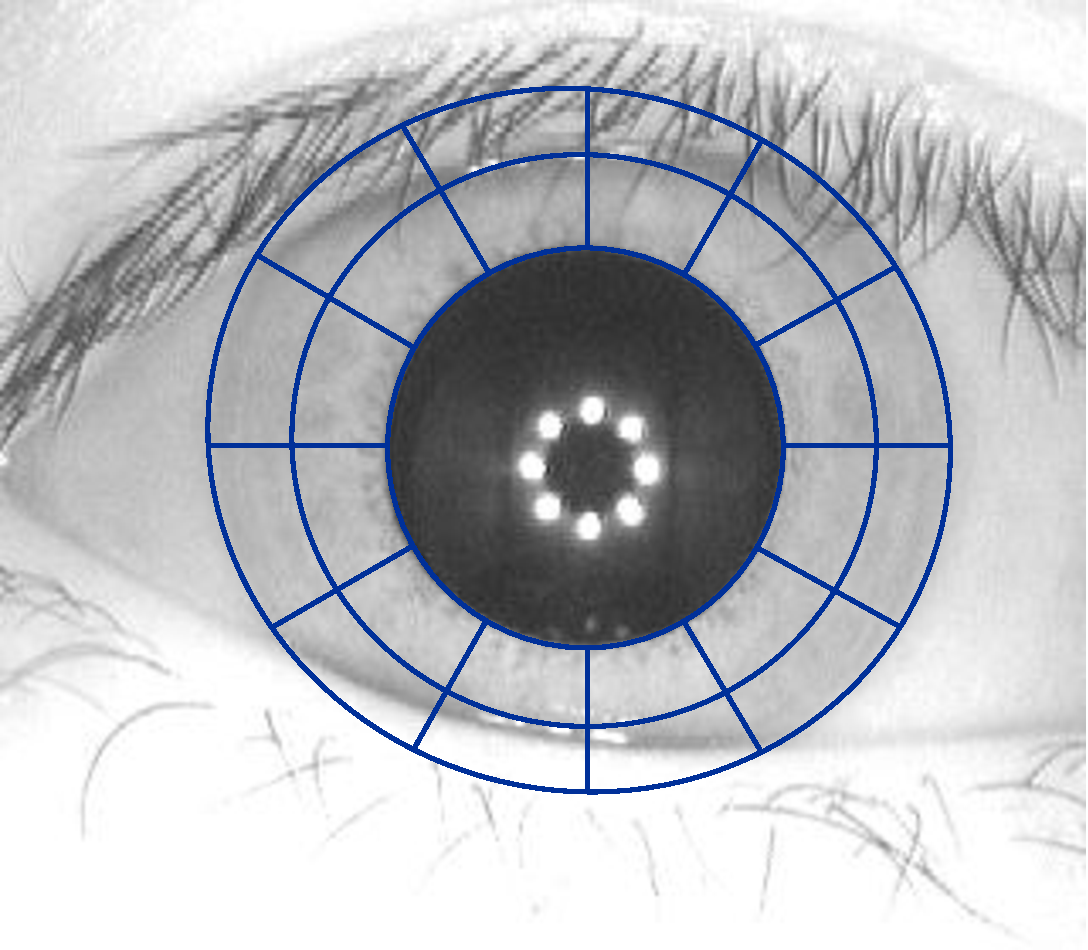
\includegraphics[width=0.6\linewidth]{figures/polar-image.pdf}
        \caption{The pupil and iris circumference ellipses define a polar coordinate system.}
        \label{fig:polar-method}
    \end{subfigure}
    \begin{subfigure}{0.5\linewidth}
        \centering
        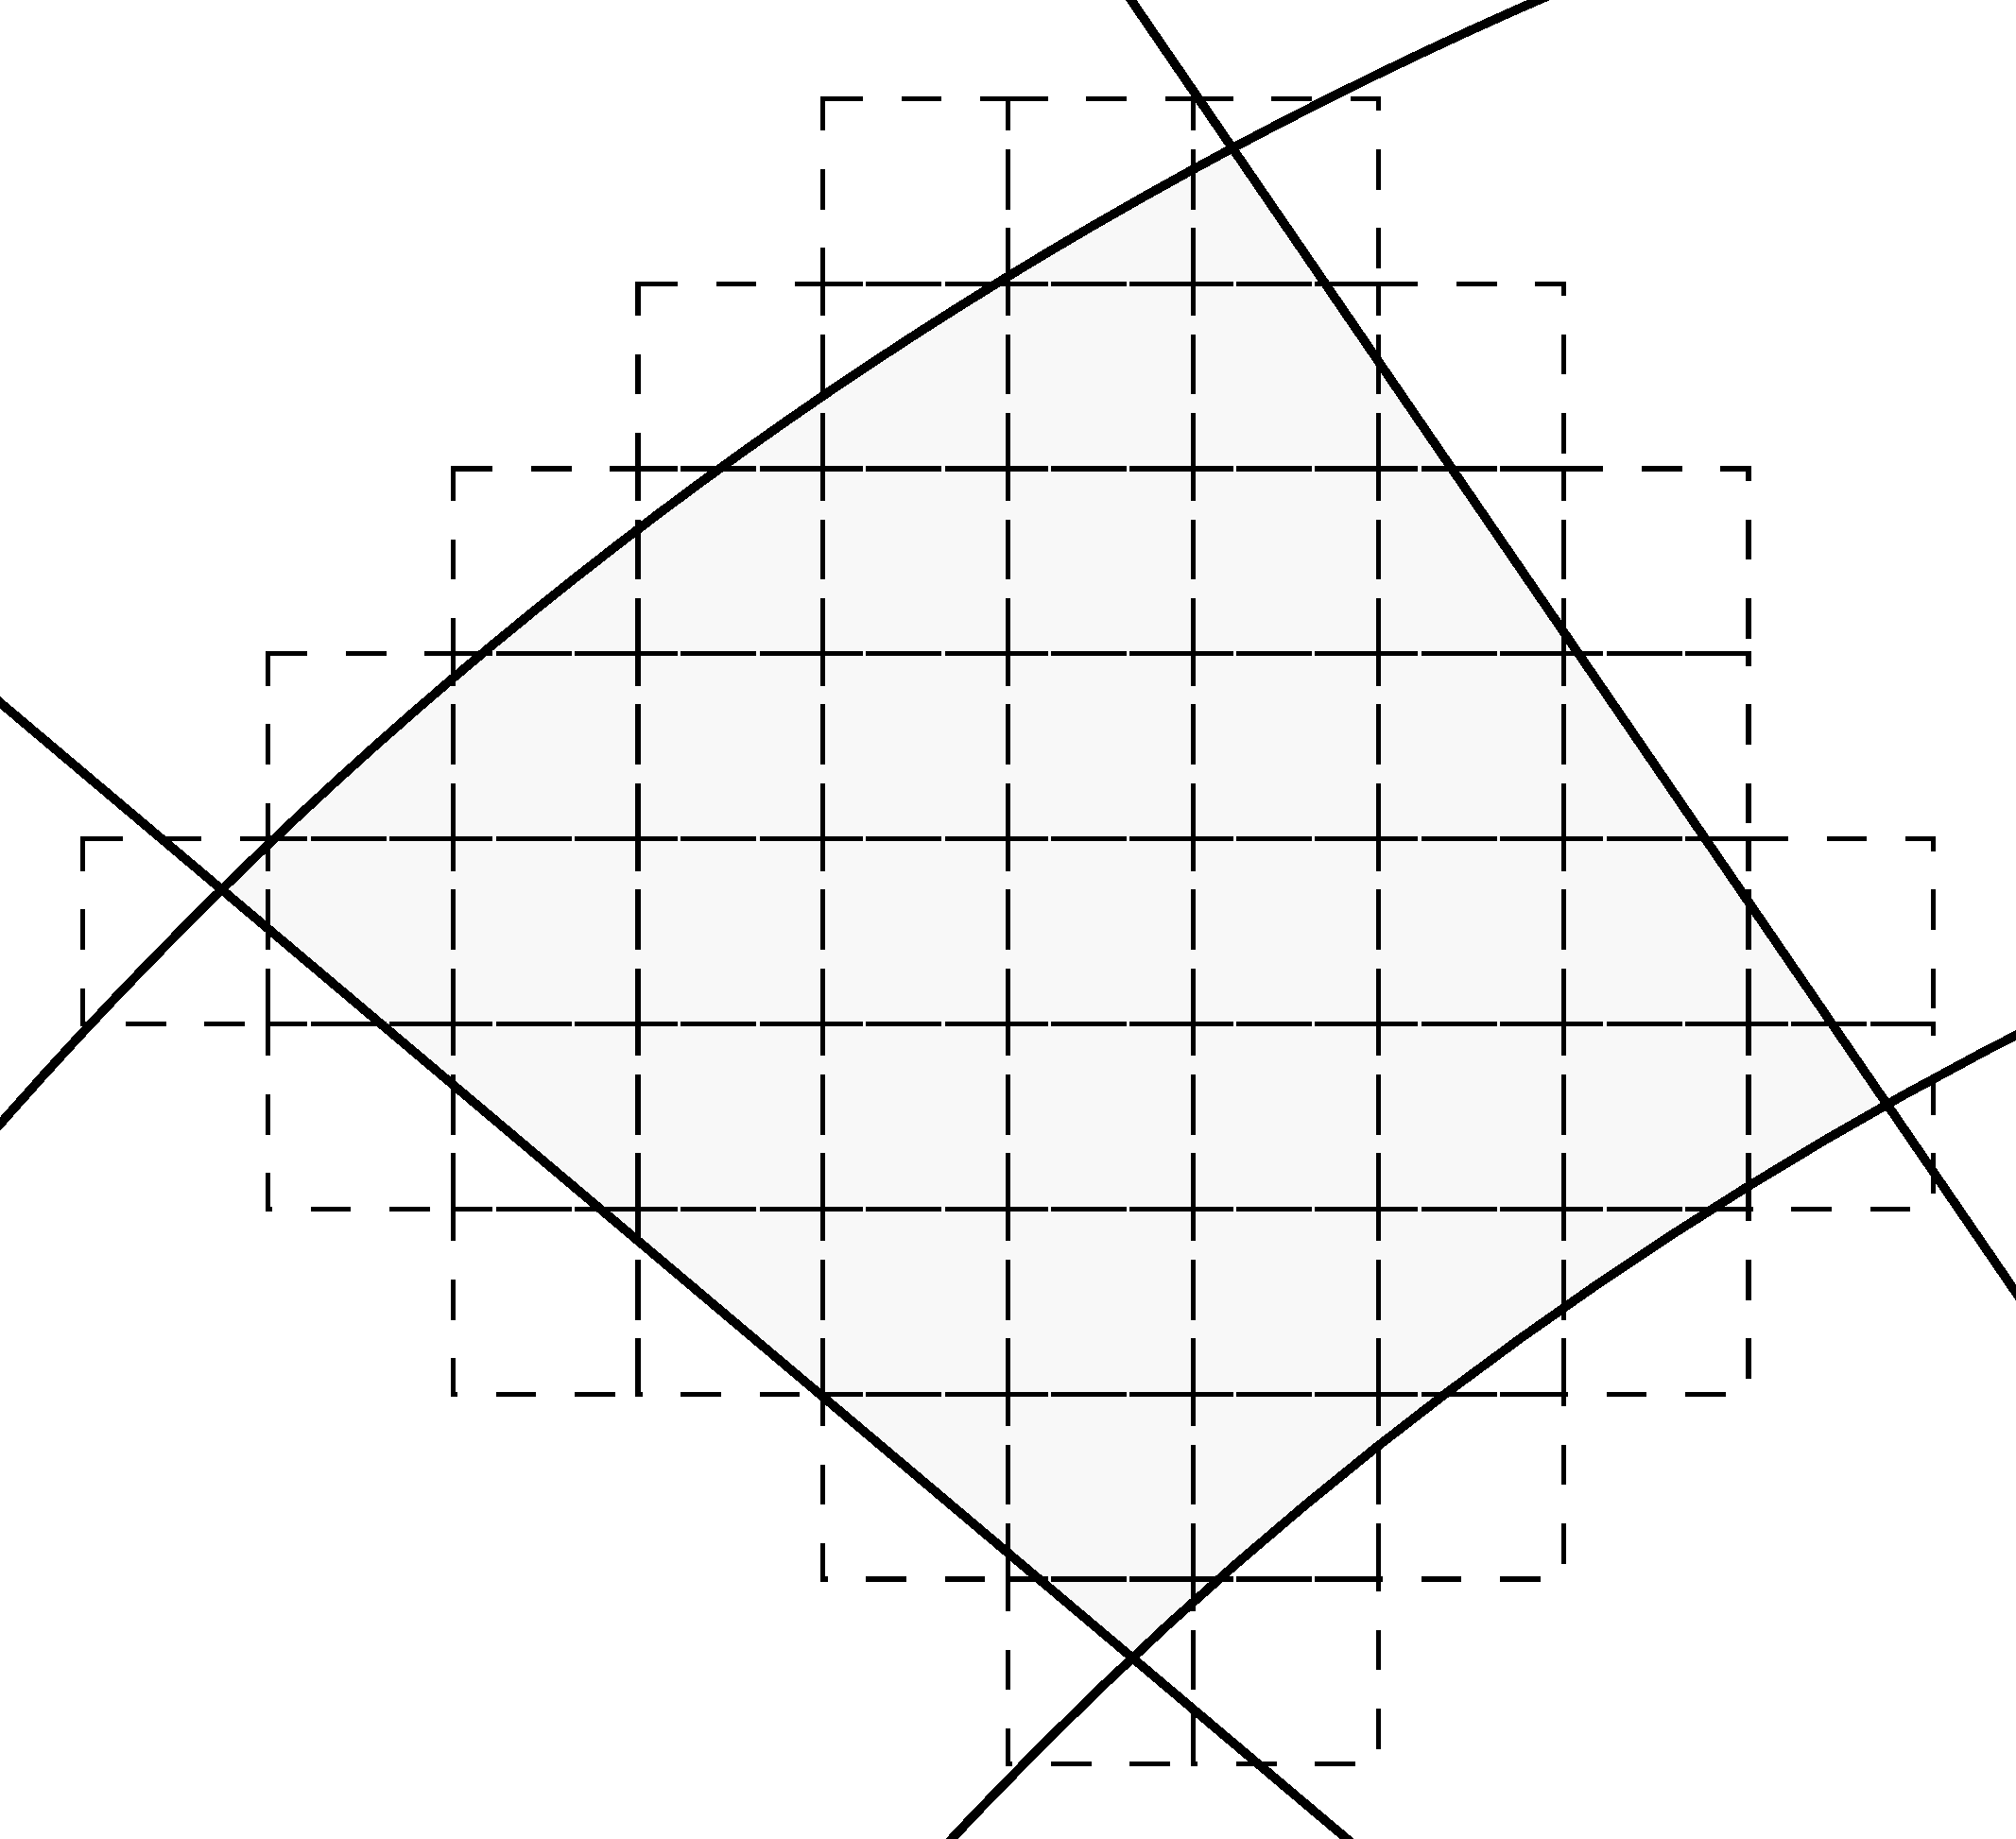
\includegraphics[width=0.6\linewidth]{figures/polar-method.pdf}
        \caption{Individual pixels in the polar coordinate system covers many actual pixels in the original cartesian space. The effect is amplified in the figure.}
        \label{fig:polar-method}
    \end{subfigure}
\end{figure}

The polar sampling method uses a particularly interesting technique. As shown in (FIGREF), the pseudo-polar coordinate system results in pixels that overlap several of the original image's pixels in strange ways. A possible solution would be to radically increase the polar resolution and use billinear sampling or similar for interpolation (REF). 

Due to the relatively slow phase calculation implementation however, I chose to keep the polar resolution low and instead opted to use a simple probabilistic sampling technique. If we denote the polar pixel region as a set $S$, each pixel in the cartesian image coordinate system is similarly sets $C_1, \dots, C_n$. The ideal pixel value at that coordinate is then:
\begin{equation}
    P(S) = \frac{\sum_{i=1}^n I_i A(S\cap C_i)}{A(S)}
\end{equation}

In other words, the pixel should take on the average value of the underlying pixels weighted by their intersecting areas. An easy way to implement this is by randomly sampling points inside $S$, adding their values, and dividing by $n$
\begin{equation}
    P(S) = \frac{1}{n}\sum_{x \sim U(S)}^n I_{x},
\end{equation}
where $U(S)$ is a uniform distribution over $S$. This method works for any size...

\begin{figure}
    \centering
    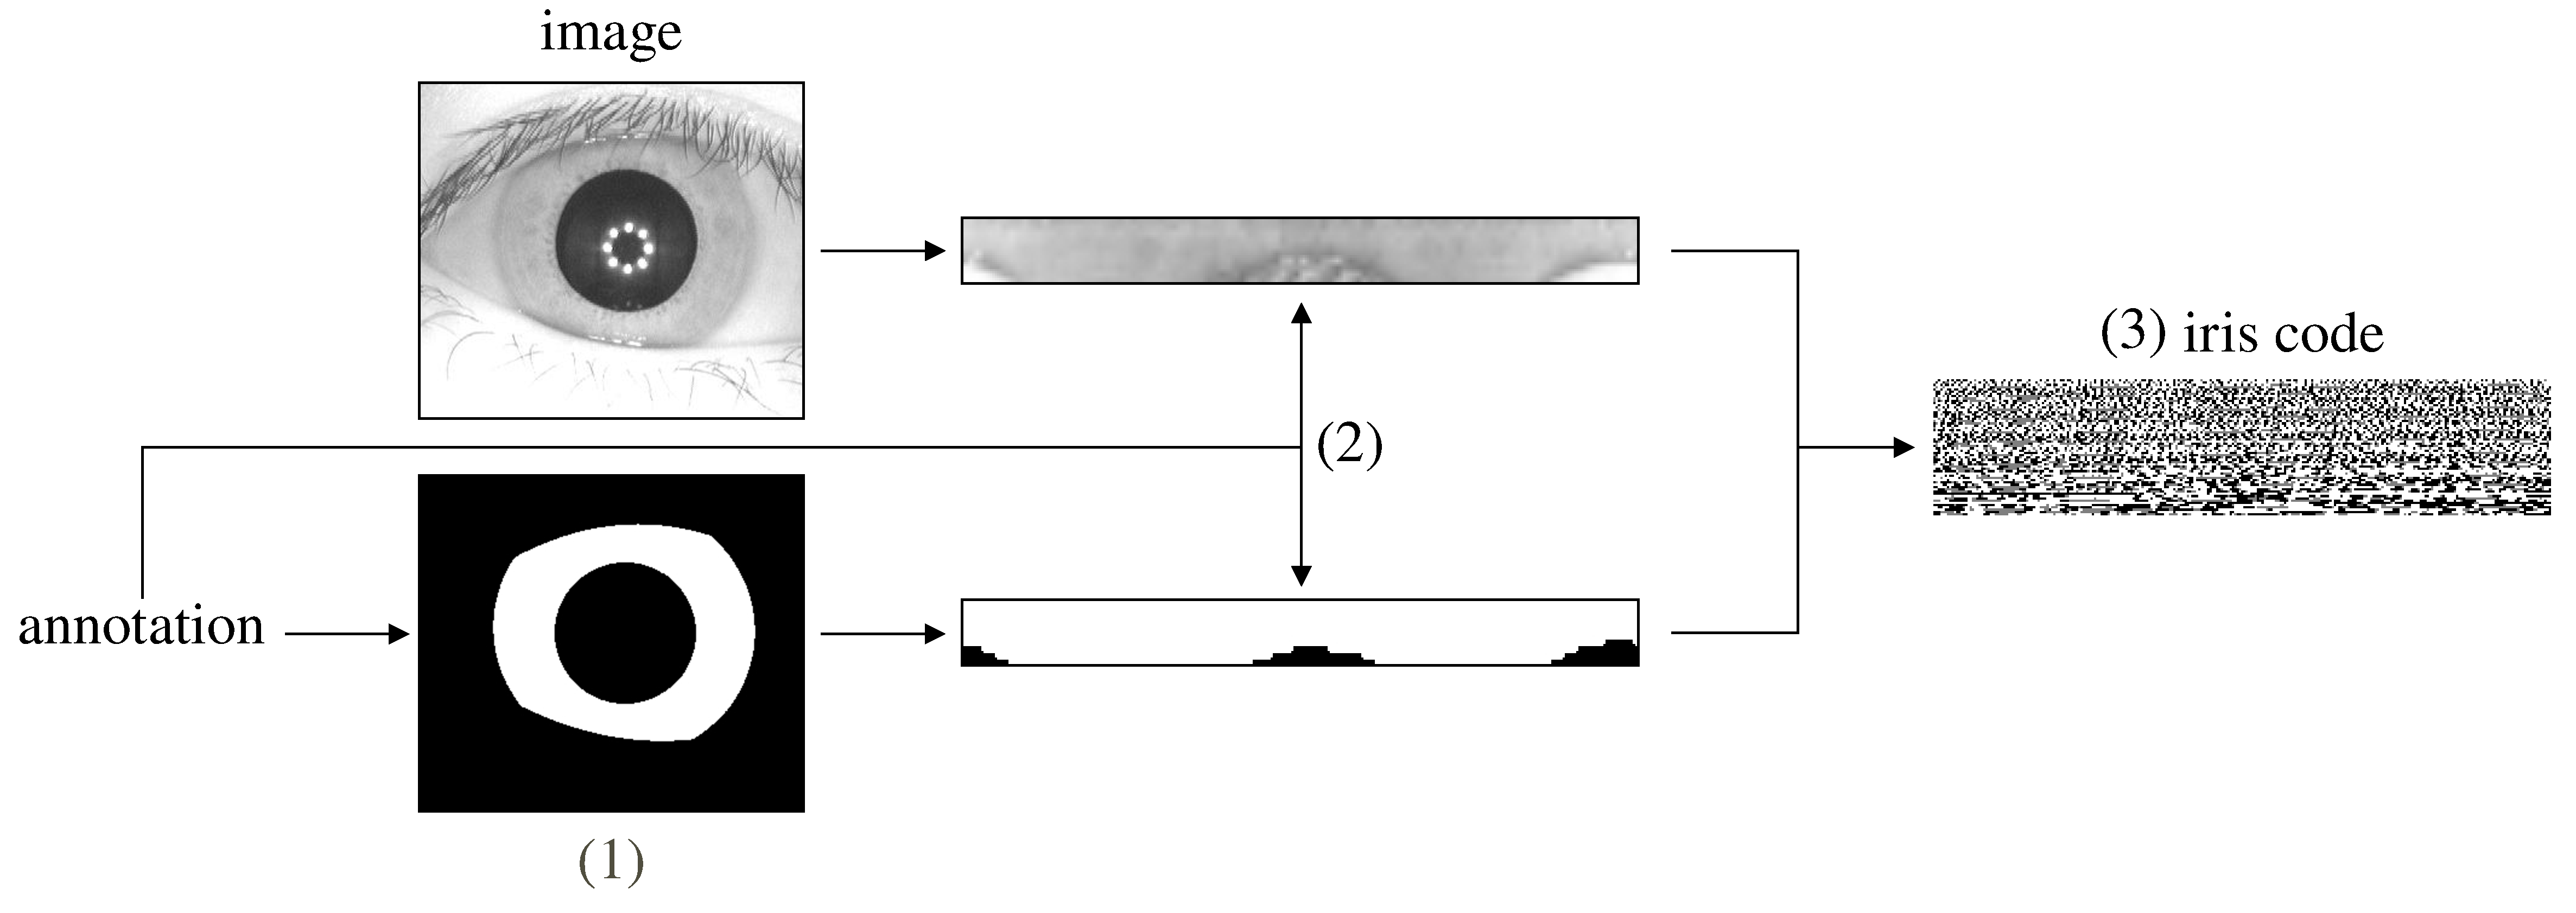
\includegraphics[width=1\linewidth]{figures/iris-code-gen.pdf}
    \caption{Iris code generation process. (1) The annotation (see text) is used to generate a binary mask of the visible parts of the iris. (2) The pupil and iris boundaries are used to create dimensionless polar projections of the iris and mask. (3) Gabor filters are applied to the polar image, quantized, and concatenated to a $16000$-element bit-vector which is the iris code. It is here visualised using black pixels for the value $0$ and white pixels for the value $1$. Pixels masked by the polar mask projection (and excluded from comparisons) are shown in grey (zooming might be necessary). }
    \label{fig:iris-code-gen}
\end{figure}

\section{Optimisation system}
Iris obfuscation has at least two objectives, one for the gaze accuracy and one for the iris recognition accuracy. This is problematic for classical optimisation where the goal is to find an extremum of a cost function with $\mathbb{R}$ as its domain. The field of multi-objective optimisation deals with exactly this kind of situation. A possible solution is to define a weighing of each sub-objective, i.e.
\begin{align}
	J^{\mathcal{O}}(I) = w_{gaze}J_{gaze}^{\mathcal{O}}(I) +  w_{iris}J_{iris}^{\mathcal{O}}(I),
\end{align}
as originally suggested by my supervisor in (REF). This approach may be suitable when sufficient knowledge about the problem makes it possible to define reasonable values for the weights. It does, however, assume prior knowledge of the relative importance of the objectives. 

Instead, this study focuses on exploring the trade-offs between various objectives over a large range of possible parameter values for each obfuscation method. In the article this is done using grid-search due to the relatively limited search space. I also experimented with a population-based method for combining multiple objectives which preserves (something).

A central idea in using these explorative methods is \textit{pareto optimality}. Pareto optimality is based on the concept that even when objectives are not comparable, it is possible to determine an ordering of the optimality of points. Figure (REF) shows an example in two dimensions. The points marked in blue are objectively better than any of the black points. Being objectively better here means that it is at least as good in every dimension and better in at least one. This is called dominance - the full definition is shown in \cref{def:dominance}. Points that are not dominated by any other point is \textit{Pareto optimal} (\Cref{def:p-optimal}). The subset of all such points of a given set is called the \textit{Pareto frontier} (\Cref{def:p-frontier}). In this example, the blue points define the Pareto Frontier.

\begin{definition}[Dominance]\label{def:dominance}
Given points $\mathbf{x}$, $\mathbf{x'}$ and an objective function $f$ with domain $\mathbb{m}$, $\mathbf{x}$ dominates $\mathbf{x'}$ if and only if
\begin{align}
 \forall i \in \{1, \dots, m\} :&\quad f_i(\mathbf{x})\leq f_i(\mathbf{x'}) \\
and \quad \exists i \in \{1, \dots, m\} :&\quad f_i(\mathbf{x}) < f_i(\mathbf{x'}).
\end{align}
In other words $\mathbf{x}$ cannot be worse than $\mathbf{x'}$ for any objective and has to be better on at least one.
\end{definition}

\begin{definition}[Pareto optimal]\label{def:p-optimal}
A point $\mathbf{x}$ in set $S$ is Pareto optimal if
\begin{align}
    \nexists \mathbf{x'} \in S: \quad \mathbf{x'} \text{ dominates } \mathbf{x}.
\end{align}
\end{definition}

\begin{definition}[Pareto frontier]\label{def:p-frontier}
The subset of all Pareto optimal points in a given set.
\end{definition}

Defining a Pareto frontier for a vector-valued objective function compresses the relevant parameter under consideration to a surface. This means that 

\begin{figure}
    \centering
    \begin{tikzpicture}
    
    \draw[thick,->] (0,0) -- (4,0) node[anchor=north west] {x axis};
    \draw[thick,->] (0,0) -- (0,4) node[anchor=south east] {y axis};
    
    \draw [red] plot [smooth cycle] coordinates {(1,1) (1,3) (3,3) (3,1)};
    \end{tikzpicture}
    \caption{Caption}
    \label{fig:my_label}
\end{figure}



\section{Filtering approaches}
We approach the analysis of separating the iris signal and the gaze signal from a pragmatic perspective. An image may be visualised as a height-map to more clearly display the individual pixel values. 

(FIG) shows an eye image and a one-dimensional slice where the light intensity is graphed as a function of the x-position. Clearly, the portion covering the iris shows relatively chaotic changes but low variance compared to the rest of the image. The pupil-iris boundary and glint-pupil boundary which are used in our gaze-estimation method are clearly identifiable since they are represented as huge changes in intensity. These sorts of examples are typically also shown when introducing image edge detection, since it clearly demonstrates the connection between rate of change, i.e. the gradient, and the presence of an edge. 

When analysing the image as a Fourier series, two important factors stand out. Firstly, the iris seems to be dominated by a low-amplitude, very random signal. This indicates a range of small to medium wavelengths and high entropy. The edge regions, which are used by our gaze algorithm, instead look roughly like square waves. A square wave requires an infinite Fourier series to be represented accurately. Because the image is effectively band-limited, it is possible to recreate it with a finite series but it still spans the whole wavelength spectrum.

This signal analysis becomes important when considering methods for obfuscation. Our understanding of how the transformations affect different simpler signals may help us find suitable methods that are more well-suited to the application.

\subsection{Measuring information in images}
The term signal is rather abstract but is typically defined as a function that encodes or contains information of interest. Signals can be defined over temporal inputs, spatial inputs, or both. In the case of eye information processes, signals such as the captured eye images may be analysed individually as purely spatially divided signals or jointly as a time series of frames. The iris pattern in either its abstract or encoded form, is only resolved spatially while the gaze signal is usually analysed as a time-series. 




When viewed as bandlimited discrete signals of two dimensions, images can be analysed structurally through the 

To measure entropy and mutual information in images, it is necessary to formulate a method for defining the image in terms of a probability distribution. Specifically, it is necessary to define a model for the image distribution and estimate it using the image itself as data.

The fundamental model is that each image can be represented by an unknown distribution $P_{img}$ of an unknown number of random variables $X^1, \dots, X^n$. A simple model is the intensity histogram which estimates a discrete distribution of intensity values assuming that each pixel is independent of each other. It can be defined as
\begin{align}
    P(I=i) = \sum_{x\in\mathcal{X}y\in\mathcal{Y}} \delta_{i, I_{x,y}},
\end{align}
where $\delta_{a, b}$ is the Dirac delta function. The downside to this approach is that no correlations between pixels are considered even though they clearly exist. For use in obfuscation measurement, this is problematic since the iris recognition methods use texture and not direct pixel intensities for detection. 

In the most general terms, the distinct features of an iris pattern represents differences in the amplitude and phase of different frequencies. Many iris algorithms of the Daugman type use spatial phase responses to calculate a robust iris code. These traditional methods generally use some form of wavelet transform to separate spatial frequency-responses (REFS). The convolutional neural-network based methods likely learn similar approaches as they have been shown to learn typical bandpass-filters like the wavelets used by Daugman (REF). 

The image derivative, defined by its two partials, has excellent properties for measuring image texture complexity. The image derivative retains all information necessary to reconstruct the original image and is therefore still a valid upper bound on information measures (REF). By defining $P_{img}$ as a joint distribution of the partial derivatives of the image
\begin{align}
    P(dx=i, dy=j) = \sum_{x\in\mathcal{X}y\in\mathcal{Y}} \delta_{i, {I_{\Delta x}}_{x,y}} \delta_{j, {I_{\Delta y}}_{x,y}},
\end{align}

Additionally, we also define joint distributions on convolutions with complex Gabor wavelets. A Gabor wavelet works as a bandpass filter, i.e. it responds only to certain frequency ranges. Defining a joint distribution over the Gabor response of a particular filter makes it possible to measure the entropy in certain frequency ranges which further... By definition however, a bandpass filter does not retain all the information in the original signal and can therefore not be used for definition of upper bounds.




\subsubsection{Filters}

\begin{figure}
    \centering
    \includegraphics[width=1\linewidth]{figures/filter_effect.pdf}
    \caption{Shows effect of applying the proposed filters. The heat-maps show the corresponding gradient histogram.}
    \label{fig:filters}
\end{figure}
Specifically, one of the previous studies tested a Gaussian filter (and optical defocus) (REF) for obfuscation based on the assumption that the lowest frequency wavelength of the pupil edge would be enough to enable robust gaze estimation. The problem with the Gaussian filter is that it is a low-pass filter, i.e. it removes high-frequency components. Since sharp edges are only sharp because of these, a Gaussian filter makes images look blurry and unsharp as a result. The effect on the image in (FIG) is shown in (FIG), where a Gaussian filter with $\sigma=5$ has been applied. Clearly, the gradient at the edge has been smoothed considerably. The reason the study still reports favourable results is that the gaze-estimation algorithm is likely robust to at least some degree of edge blurring.

A smarter approach is to consider not just the spatial neighbourhood but the intensity as well. 
\section{Experiments}
This work focuses on a detailed analysis of the effect the proposed obfuscation methods have on the concurrent goals of iris obfuscation and gaze estimation over a wide range of parameter values. Because iris recognition performance is computationally expensive, the analysis is divided into two separate experiments, one for providing detailed information on the effect of obfuscation for a large number of parameter configurations, and one for providing complete ...



The proposed methods have been extensively evaluated on a number of relevant metrics and datasets (which ones?)...... The results provide a clear image of the effectiveness of the individual methods and provide us with enough detail to help us understand how they affect gaze estimation and iris recognition.

Two experiments have been performed, (1) a systematic search of filter parameters and their influence on utility, security, mutual information, and other metrics, and (2) test of iris recognition performance on the full dataset + maybe some additional gaze tests?


For the experiments we used different datasources for gaze estimation and iris recognition in order to provide favourable conditions for iris recognition. The dataset used for iris recognition, CASIA IV, is generally considered easy for iris recognition, which is good in this case since it is exactly the opposite when the goal is to prevent correct recognition.


\subsection{Eye tracker setup}



The gaze dataset was recorded using a remote camera placed close to the eye to simulate the location on head-mounted eye trackers. A chin rest was used for keeping the head stable during recording. The participants were asked to fixate on a number of targets on a screen placed approximately 60cm from their head. A single infrared LED provides a glint used for normalisation. A set of 25 calibration images and 50 test images were recorded for each participant, with the calibration samples being placed in a regular grid and the test images being sampled from random uniform distributions.



\paragraph{Gaze estimation}

The gaze model used is a 2nd degree polynomial using a pupil-glint vector as its normalised input. The method requires detection of the pupil which is done by the DeepEye network (REF) and detection of the glint which is done using image thresholding and BLOB detection. 

\subsection{Iris recognition}

For iris recognition, we made an iris recognition algorithm that models Daugman's method as closely as possible, i.e. it uses a quantisation of phase over the iris region as the identifying code. The \emph{hamming distance} between codes is used to model distributions for matches and non-matches respectively, which are finally used to select a threshold used to determine, whether a comparison should be accepted or discarded. As in Daugman's articles, the complex 2d Gabor function is used as a bandpass filter. Phase quantisation is applied to the result to produce two bits of iris code for each Gabor application location. We ended up using 4 scales and 6 angles per scale. Since gabor filters do not have an orthogonal basis, these filter banks are selected empirically. 

Base iris recognition performance is shown in (FIGREF) and is acceptable compared to other similar algorithms. 
Without obfuscation, the algorithm performs favourably compared to many other iris recognition algorithms (refs) and is within a few orders of magnitude of the original. Larger datasets and a direct comparison would be needed to accurately determine the real-world performance. 

However, the process of determining iris recognition performance on a given dataset requires many samples to produce reliable results. Specifically, given $n$ comparisons of different source irises and $m$ comparisons of equal irises, the false acceptance rate can only be determined in increments of $1/n$ and the false rejection in increments of $1/m$. Assuming the distributions approximate normal distributions (Daugman REF), their means and variance estimators have variance $Var(\bar{X})=\sigma^2/n$ and $Var(S_n)=\sigma^4/(n-1)$ respectively .... and so on...

We therefore choose to only perform actual iris recognition for a few select parameters for each filter. The iris recognition comparison uses the CASIA IV dataset (REF). A subset of $2,600$ images which have been manually segmented are used (REF). This removes any influence an iris detection mechanism might have and thus provides optimal conditions for effective iris recognition. Additionally, the dataset itself is relatively easy, which purposefully makes obfuscation as difficult as possible and thus should increase our trust in the results.





\subsection{Parameter experiment}
A grid-search was performed for each obfuscation method with linearly spaced parameter values. For each parameter configuration a selected number of metrics were evaluated on samples drawn from the respective iris, gaze, and pupil-centre datasets using the obfuscation and transformed using the relevant obfuscation method. Searching the parameter space in this systematic manner has the advantage of presenting us with a more complete picture of how the various metrics react to parameter changes over the whole spectrum of possible values. Parameter configurations and precise metric descriptions are found in appendix??. 

Importantly, the random sampling makes the results stochastic as well, which is why these results are not used for evaluation directly. This necessary trade-off allows a significant increase in the number of parameter values tested which provides insight into how the different methods work and compare.

\subsection{Evaluation experiment}
The evaluation experiment tests iris recognition performance on the complete set of $2,600$ iris images. This results in $xx$ possible code comparisons for each test. Two testing methodologies are used for evaluating the obfuscation methods. For both, the iris codes for the entire dataset are computed for a selected number of parameter configurations for each obfuscation method.

The first test compares the iris codes from the obfuscated images with the original iris codes derived from the unmodified images. The resulting distances thus reflect data from a situation where the obfuscated data is checked against an existing iris database for matches. 

The other test compares the obfuscated codes internally and therefore reflect the possibility of constructing a new iris database from obfuscated images and using it for subsequent identification. 

Both tests are equally relevant. The former determines whether the obfuscation methods can be used as safeguards against being recognised using a known reference while the latter determines if obfuscated images can related ..... Both situations are problematic as...

\chapter{Discussion}
This chapter is an extension to the article with additional analysis of the results and a more thorough discussion of how the results support the proposed model and what insights the results give to support its use for other applications.

\section{A detailed look at obfuscation method information}
\begin{figure}
	\centering
	
	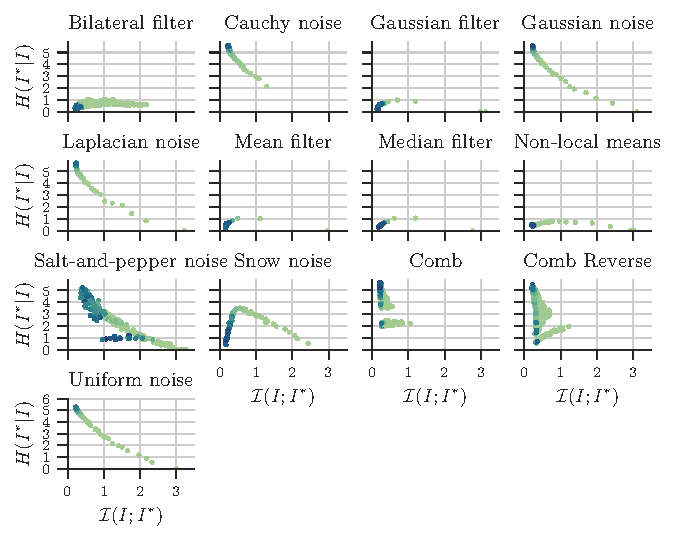
\includegraphics[width=1\textwidth]{figures/results/individual}
	
	\caption{Plot of mutual information and conditional information response for individual filters. Note that these distributions are estimated from the entire image, producing less noisy results than the ones presented in the article.}\label{fig:individual}
\end{figure}

\Cref{fig:individual} shows mutual information and conditional entropy for each filter separately. This makes the distinction between them even more noticeable. 

The noise methods, except snow and salt-and-pepper, all follow an almost straight line, "converting" mutual information into conditional entropy. \Cref{fig:individual-entropy} is similar, but with the output image entropy as its x-axis. From this figure it is clear that for all noise methods, the increase in conditional information is roughly proportional to the increase in entropy, but not at a one-to-one scale. As shown in \cref{eq:entropy-law}, this necessitates a loss in mutual information, i.e. $\mathcal{I}(I^*;I) = H(I^*) - H(I^*|I)$. Since the entropy and conditional entropy are roughly linearly correlated for the noise-based methods, we have $H(I^*) \approx \alpha H(I^*|I) + H(I)$ and as a consequence, the mutual information can be expressed as a function of the conditional entropy and the entropy of the original image 
\begin{align*}
\mathcal{I}(I^*;I) \approx (\alpha-1)H(I^*|I) + H(I).
\end{align*}
This is of course only an approximation.

The snow method has a sudden drop in conditional information which is caused by its definition. At low densities, snow increases conditional entropy because the randomly placed pixels adds high gradient components. At higher densities however, the fact that only the value $127$ is used for pixels starts to decrease the entropy significantly. %The uniform snow method is susceptible to the same effect when gaussian variance is low and \todo{what about this?}

\begin{figure}
	\centering
	
	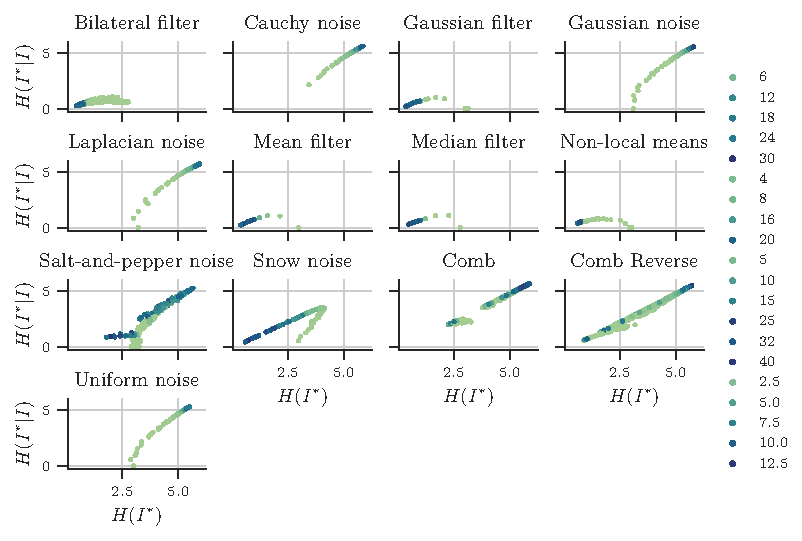
\includegraphics[width=1\textwidth]{figures/results/individual-ent}
	
	\caption{Plot of entropy of the obfuscated images and conditional information response for individual filters.}\label{fig:individual-entropy}
\end{figure}

The filter-based methods behave as explained in the article and mainly impact mutual information. The combination methods, and especially Comb, is worth investigating further. \Cref{fig:comb} uses the same axes as \cref{fig:individual} but displays only data from the Comb method and with the colours indicating the three parameters in the respective plots. The scale parameter, $\gamma$, correlates directly with the value of conditional entropy as expected. The generally lower mutual information values are likely caused by a narrower band of parameters used for the experiment due to time considerations. It shows that the diagonal bands visible in the figures corresponds to the response caused by the bilateral filter. It correlates highly with the color variance parameter $\sigma_c$ but is seemingly independent from the spatial parameter $\sigma_s$. This effectively means that only small values of $\sigma_s$ is needed.

\begin{figure}
	\centering
	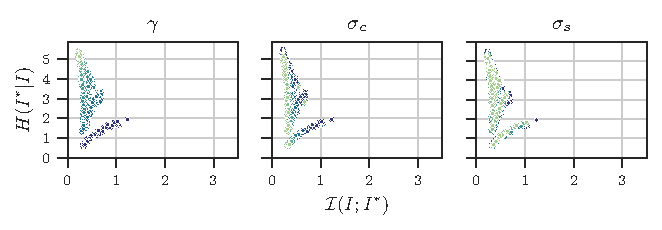
\includegraphics[width=1\textwidth]{figures/results/comb}
	\caption{}\label{fig:comb}
\end{figure}
\todo{Discuss camera effects}

\subsection{Filters and gradient entropy}
Although the approach to filtering has been argued extensively in the article, it did not show how visually appropriate the gradient entropy is compared to a simple intensity entropy. \Cref{fig:delentropy} shows a number of sample images for which both the intensity histogram and gradient histograms have been calculated. It is visually very clear how the gradient histogram and its entropy corresponds with the visually perceived image complexity.

\begin{figure}
    \centering
    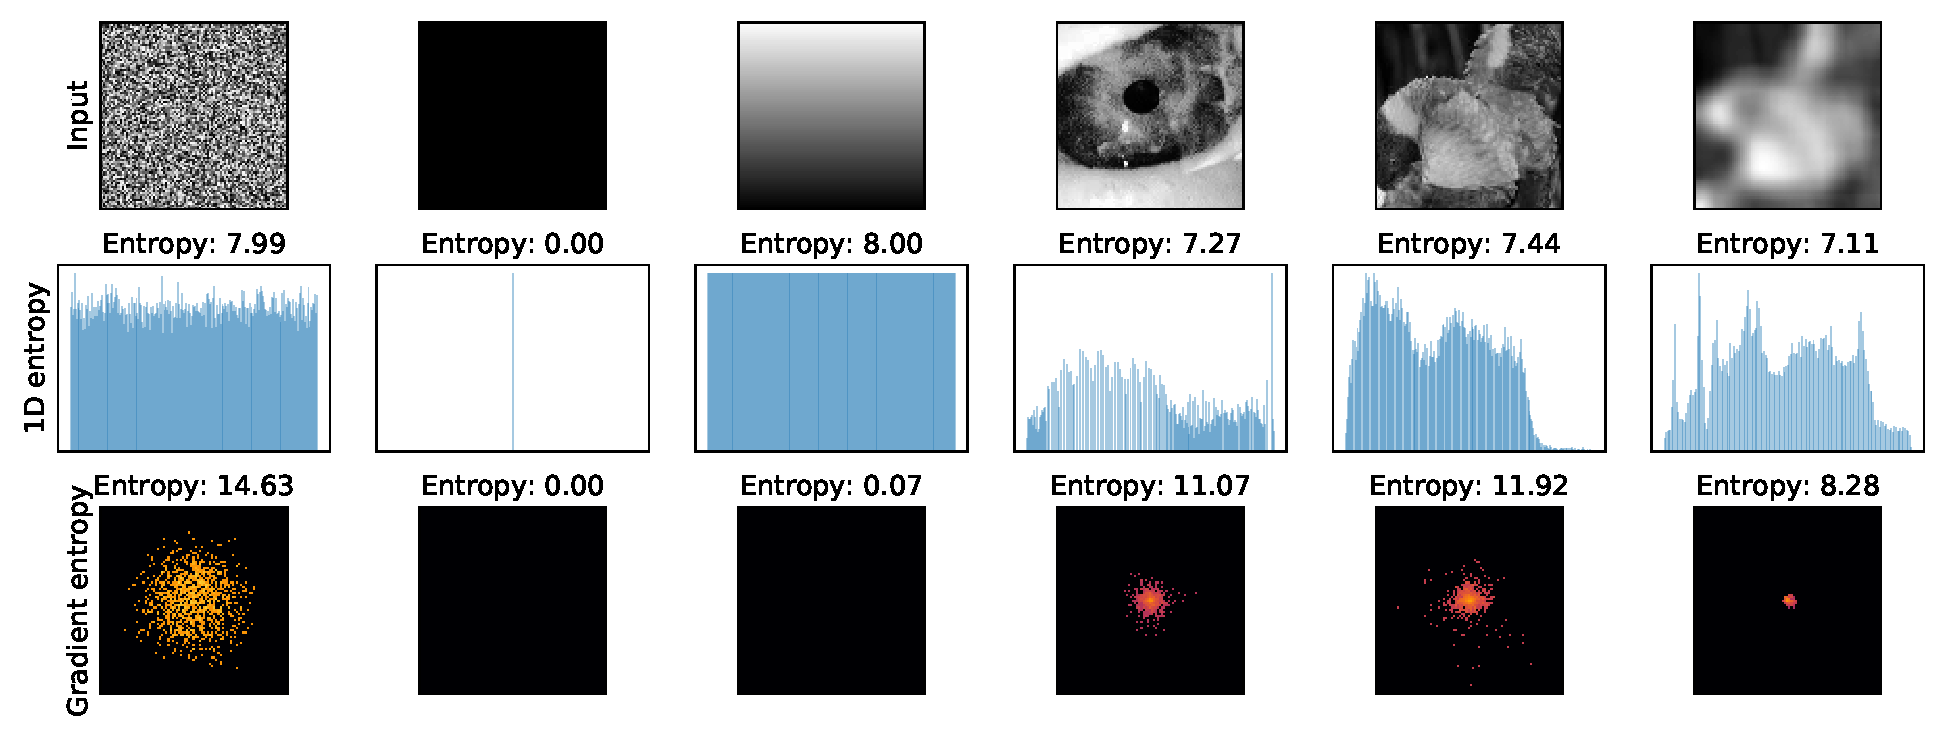
\includegraphics[width=1\linewidth]{figures/results/delentropy}
    \caption{Comparison between entropy of intensity and gradient histograms for a number of image samples.}
    \label{fig:delentropy}
\end{figure}

Sample applications of the proposed obfuscation methods are shown in \cref{fig:filters} where the same visual correlation is still clearly present. The Comb method is also visually indicative of its effectiveness as an obfuscation method because of the clear blurring of eye details while retaining a layer of noise. The parameters used in this example are exaggerated to increase the perceivability of the effects.

\begin{figure}
    \centering
    \includegraphics[width=0.85\linewidth]{figures/results/filter_effect.pdf}
    \caption{Shows effect of applying the proposed filters. The heat-maps show the corresponding gradient histogram.}
    \label{fig:filters}
\end{figure}


%Specifically, one of the previous studies tested a Gaussian filter (and optical defocus) \parencite{BRENDAN_BLUR} for obfuscation based on the assumption that the lowest frequency wavelength of the pupil edge would be enough to enable robust gaze estimation. The problem with the Gaussian filter is that it is a low-pass filter, i.e. it removes high-frequency components. Since sharp edges are only sharp because of these, a Gaussian filter makes images look blurry and unsharp as a result. The effect on the image in (FIG) is shown in (FIG)\todo{do it}, where a Gaussian filter with $\sigma=5$ has been applied. Clearly, the gradient at the edge has been smoothed considerably. The reason the study still reports favourable results is that the gaze-estimation algorithm is likely robust to at least some degree of edge blurring.

%A smarter approach is to consider not just the spatial neighbourhood but the intensity as well. 

\section{Eye information process model generalisation}\todo{ikke klart hvem der siger det...}
For the model and methodology presented in this thesis to be useful, it has to be relevant to the way this category of problems are perceived and to how they are evaluated. For the specific application of iris obfuscation, this has been argued extensively in the article. At an abstract level, the model is used to understand the problem of iris obfuscation and for proposing reasonable and interesting solution candidates. At a concrete level, the information-based metrics and methods derived for calculating them for images showed a high correlation with the observed iris recognition accuracy.

The definition of the model itself as a Bayesian network or as a communication system is an expression of the similarity of image and signal manipulation operations and, by extension, of obfuscation methods in general. The optimisation goal defined for iris obfuscation is thus the same for any other obfuscation problem. The gaze signal itself contains information that has been shown to reveal multiple properties of the recorded subject and is therefore an obvious candidate for using the model. The model and methodology presented here can be applied directly. 

If applied to other problems, results become easier to analyse and compare, and the methodology itself will develop which might provide additional insight into already published material. 

\section{Differential privacy}
Differential privacy is too strict to be a realistic measure for proving privacy bounds for obfuscation tasks. Specifically, only low privacy-bounds are achievable by the application methods proposed so far in the literature. I here present the argument that this is caused by the properties of differential privacy when applied in this domain. Differential privacy is simply a measure of how much a random function impacts the predictability of changing a single element in a set of data points, e.g. an image. Formally, a random function $\mathcal{K}$ is $\epsilon$-differentially private if
\begin{align}
	P[\mathcal{K}(D_1)\in S] \leq \exp{\epsilon} P[\mathcal{K}(D_2)\in S],
\end{align}
for all subsets $S$ of the image of $\mathcal{K}$ and all datasets $D_1$, $D_2$ that differ in at most one element \parencite{dwork2006differential}. In other words, a differentially private function decreases the output's dependence on individual data points since this dependence can be used to infer the original data points.

Differential privacy measures for images have been proposed by \parencite{fan2018image}. Importantly, their extension from single pixel changes to neighbourhoods come with a proportional increase in $\epsilon$ for the same amount of randomness, i.e. for a neighbourhood of $n$ pixels, the privacy should be $\epsilon/n$ to achieve the same level of protection as when a single element is changed. The solution presented in this study suggests an aggressive downsampling using averaging to achieve reasonable levels of noise. Specifically, for an image with pixel intensities in the range $0-255$, and using laplacian noise, the scale parameter is $\frac{255n}{b^2}$ where $b$ is the side length of grid cells defining regions to be averaged. Since laplacian noise has a variance of $2s^2$ where $s$ is the scale, even a low-resolution image of $100\times 10$ pixels (the size used for polar iris images in this work) would require laplacian noise with a variance of $\approx 130\times 10^9$ thus rendering the image practically unusable.

The method proposed in \parencite{BRENDAN_SNOW} does, however, use a weaker form of differential privacy allowing an extra constant term $\delta$ which signifies a probability of leaking information. They prove that $\delta$ has a maximum of $0.5$ for the snow method which means that each pixel has $50\%$ chance of a leak. However, as presented in \cref{sec:methods}, the method can easily be defeated if multiple samples are available. Additionally, even with a single sample, the method shows only moderate effectiveness at preventing recognition with high precision at low recall values. 

In conclusion, differential privacy is not suitable for determining the security of obfuscation methods due to their high sensitivity and the large areas of pixels that need to be secured. As a final note, this criticism does not concern the aggregation based attempts at differential privacy in eye-tracking mentioned in the article. %Instead it is 
 differential privacy has been shown to be highly effective in other eye-tracking privacy tasks where aggregation is involved \parencite{differential-general, differential-general-two}.

\todo{Try to add the rest here}
% Instead, definitions should be derived from a

%\begin{definition}[Privacy]
%Let $S$ be an eye information signal and $\bar{S} \subseteq S$ a subset describing the sensitive data. 

%Let $\mathcal{A}$ be an arbitrary function for inferring 
%Given an arbitrary information extraction function $\mathcal{A}$, an obfuscation function $\mathcal{O}$, and a signal $S$, the privacy strength of $\mathcal{O}$ is defined as
%\begin{align}
%	P[\mathcal{A}(\mathcal{O}(S)) \cup \bar{S} \neq \empty] \leq \rho,
%\end{align}
%for an arbitrary threshold $\rho$ and for any $\mathcal{A}$.
%\end{definition}
























\section{Discussion}
